\section{Conceptual Modeling in XR}
\label{sec:background-conceptual}

Bille et al.~\cite{bille_conceptual_2007} define \emph{Conceptual Modeling} as \textit{the activity of building a model of the Universe of Discourse (UoD) in terms of concepts that are familiar to domain experts and free from any implementation details}. The Universe of Discourse is the slice of the world we want to explore. 
A proper conceptual model aids the understanding of the tasks that constitute the system \cite{norman_design_2013}. Moreover, there is a difference between the model of the system as perceived by the user and the system itself, and the more they deviate from each other the less they can be considered acceptable models \cite{rosson_usability_2002}. The expectations of the designer of a model do not always correspond to those of the user. The former creates models shaped by diagrams and analyses, while the latter creates models shaped through experiences and interactions \cite{laviola_jr_3d_2017}. 

Other pros, besides the intuitiveness of the concepts and the clarity of the information for those who have to use it, are addressed in \cite{bille_conceptual_2007}. They include the possibility of isolating parts of the domain, supporting dialogue between the figures involved and, finally, providing a high-level, rapid and convenient debugging. 
The need to build conceptual models is rooted in the context of database systems, whose increasing complexity has led experts and non-experts to consider and model all information and requirements, useful for implementation, even before acting on the physical components \cite{connolly_database_2005}.

Conceptual modelling has become increasingly popular in the field of design engineering, which is the reason why it is discussed in this thesis in relation to the latest technologies. 
The arguments researched in the literature that led the authors to develop conceptual models in VR and AR are numerous, basically deriving from the abstraction of the application to be developed from the implementation layer \cite{de_troyer_conceptual_2007}. The development of XR, VR and AR applications should address the design of the components of an experience, before proceeding to the implementation phase. This step, indeed, requires a background knowledge of the technologies that belongs only to the most experienced programmers and not always to the experience designers. 
The translation of real-world concepts, which we want to translate into the virtual/augmented world being built, is challenging and time consuming if these concepts are not modelled at a high level. By introducing a level of design that precedes the writing of the code, complexity is reduced, interventions are more immediate, resources and time are optimised, communication is better within the team because non-experts are also involved \cite{coninx_vr-demo_2006}. 
Moreover, behind the development of an application there are professionals who contribute to the creation of the contents and the introduction of conceptual models allows even those who do not have a technical background, related to programming or 3D design, to understand the logic of the application \cite{walczak_structured_2008}. 
In addition, many authors address the problem of solution re-usability, which becomes difficult when applications follow domain- or hardware-specific models, guidelines and tools \cite{figueroa_conceptual_2006}. 

\subsection{Conceptual Models}

Numerous studies in the literature present conceptual models in AR and VR environments. A brief overview of the works analysed is given, reported according to the technology used (VR, AR, MR) since they have different features and interaction paradigm.
Recurring terminology in this section includes concepts like 'high-level modelling', i.e. modelling that abstracts from application development and whose understanding does not require a technical background. Next we will discuss 'interaction techniques', defined as a \textit{way of using a physical input/output device to perform a generic task in a human-computer dialogue} \cite{foley_computer_1990} that in this context are applied to the technology involved. 'Multimodal interactions', on the other hand, include ways of relating to and communicating with not only physical but also Virtual Environments (VEs) \cite{bourguet_designing_2003}. 

% VR
The last two decades have seen the rise of frameworks for VR applications. Latta et al.~\cite{latta_conceptual_1994} proposes a VR system with two perspectives: a human-centred view that characterises participants and their muscular and perceptual systems, and a technical view that defines both the real and simulated participatory environment within which humans interact. The stimuli generated by the environment trigger sensations to which humans respond through actions that are recognised by the sensors of the environment itself. A confection model (\autoref{fig:latta}) is used to relate participants to the real environment, and its components handle the interface control functions. 

\begin{figure}[h]
    \centering
    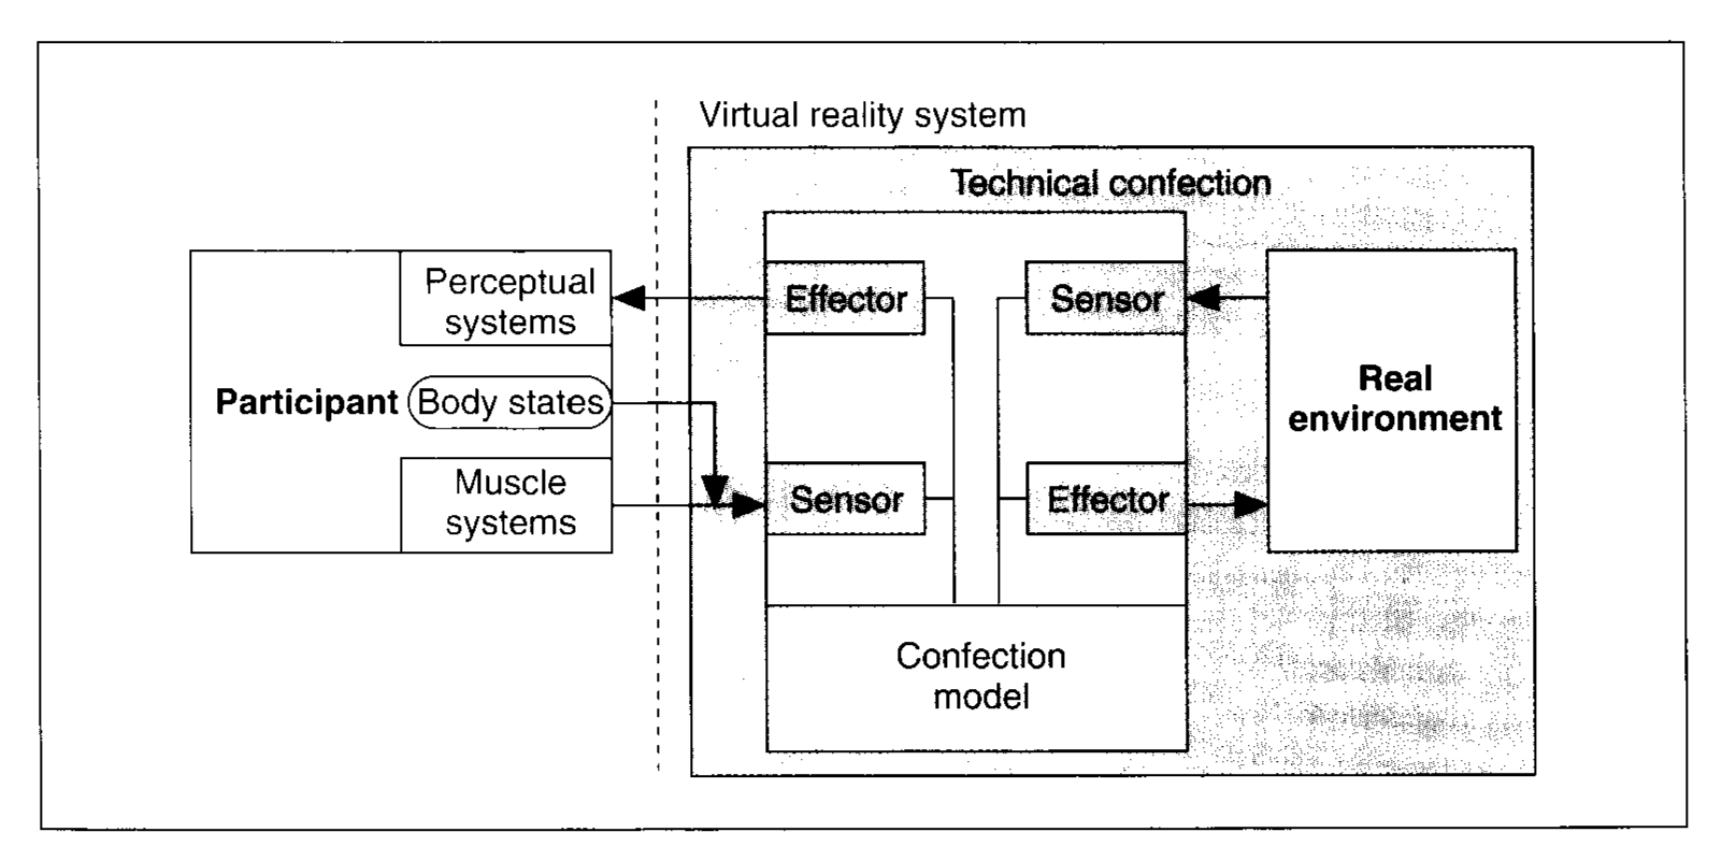
\includegraphics[width=\textwidth]{Figures/Background/models/latta.png}
    \caption{Conceptual Models - VR System}
    \label{fig:latta}
\end{figure}

More recent research describes the interaction techniques required to perform tasks involving the use of 3D interfaces performed by users. In this regard, the book of LaViola Jr et al.~\cite{laviola_jr_3d_2017} explains the 3D interaction techniques applicable to different devices by organizing human tasks in selection and manipulation, travel intended as navigation, wayfinding, ending with tasks related to system state change and symbolic input. No code or pseudocode translation is attached to the extensive description, thus the interpretation and development choices are up to the implementer. 

Facilitating the developer's workload is one of the main arguments addressed in \cite{coninx_vr-demo_2006}, which introduces \textit{VR-Demo}, an approach that allows to design high-level \gls{VE} applications with a supporting tool. The logical structure separates the modelling of the VE and the behaviour of its components from user interactions. De Troyer et al~\cite{de_troyer_conceptual_2007} introduce a conceptual design step into the development process, allowing to achieve a level of abstraction that would enable non-experts to build VR applications. The proposed method, VR-WISE (\autoref{fig:detroyer}), contemplates a three-phase development cycle, one more than VR-DEMO. The first phase consists of \textit{conceptual specification of the domain and behaviour and the actual virtual world}. The second stage is the \textit{mapping of the domain and world} and the last is the \textit{generation} of the code. Despite the detailed modelling of concepts and behaviours, the work lacked the modelling of interactions, that is addressed in VR-DEMO. To support the interactions Berge et al.~\cite{berge_towards_2014} use a collection of links to connect the sub-tasks the user has to perform with the elements of the 3D VE involved in the task to be accomplished (\autoref{fig:berge}). The resulting analytical framework consists of two tree structures, one decomposing the user tasks into sub-tasks and an interactive scene graph showing the hierarchy of 3D objects, lights and virtual cameras. 

\begin{figure}[h]
    \centering
    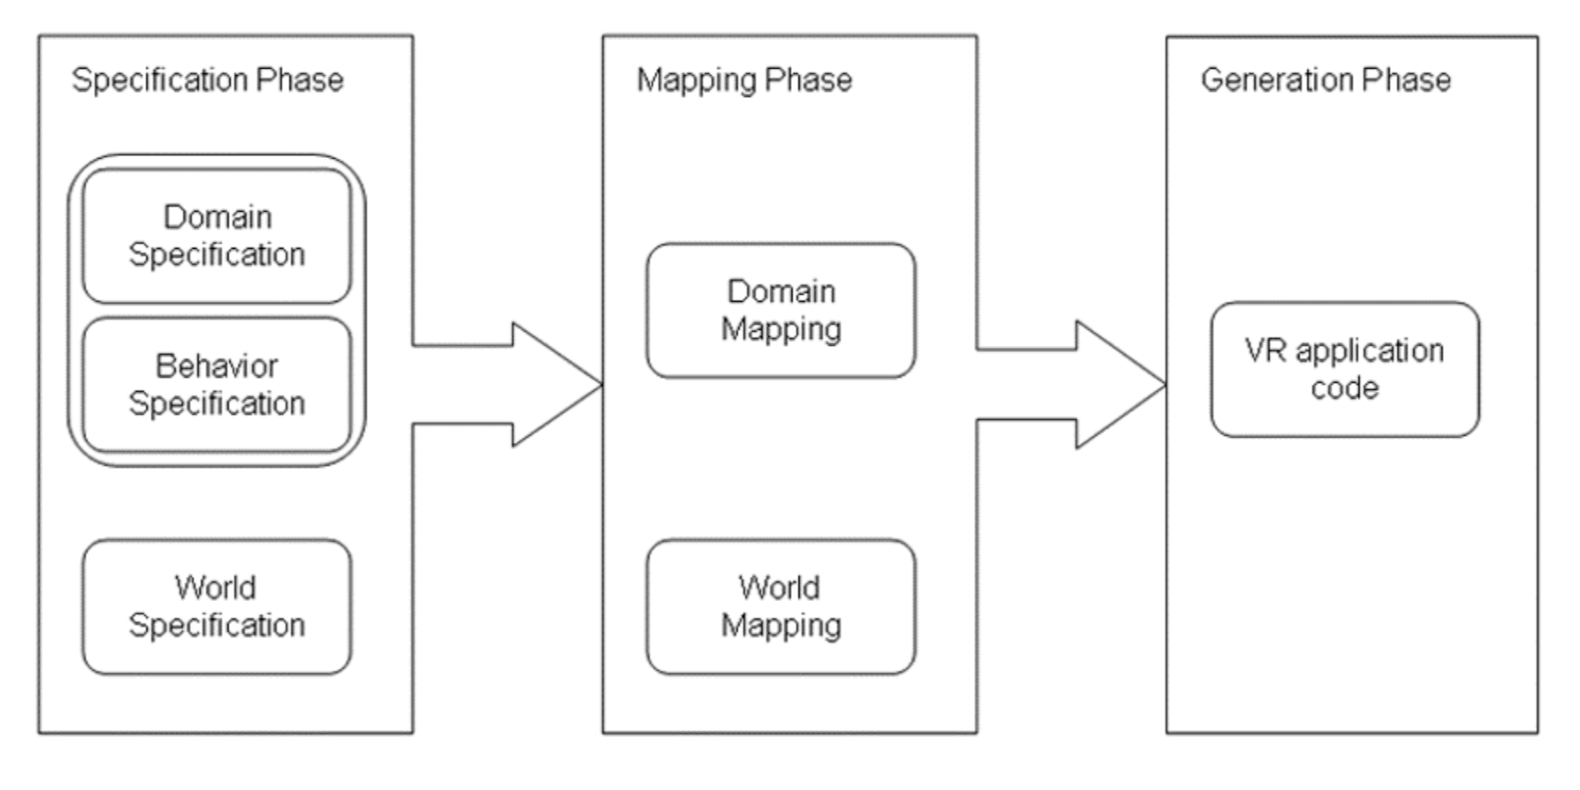
\includegraphics[width=\textwidth]{Figures/Background/models/detroyer.png}
    \caption{Conceptual Models - VR-WISE}
    \label{fig:detroyer}
\end{figure}

\begin{figure}[h]
    \centering
    \includegraphics[width=\textwidth]{Figures/Background/models/bergè.png}
    \caption{Conceptual Models - Analytical Framework}
    \label{fig:berge}
\end{figure}

% AR
As far as AR modelling is concerned, the work of Pendit et al.~\cite{chandini_pendit_conceptual_2015} is devoted to cultural heritage projects and seeks to involve the visitor in the activities, to give them positive feelings, to satisfy their needs so that the overall experience is enjoyable. The proposed conceptual model (\autoref{fig:chandini}) identifies 3 structures containing a large number of elements. The first structure includes the hardware components and the process phases of development, the second includes a set of functions that guide the visitor through the Cultural Heritage site, and the third includes the components that make learning enjoyable such as activities, interaction, personalisation and games. The intersection between the structures is a set of elements such as 3D Model, 3D Character, Text, Image and so on.

\begin{figure}[h]
    \centering
    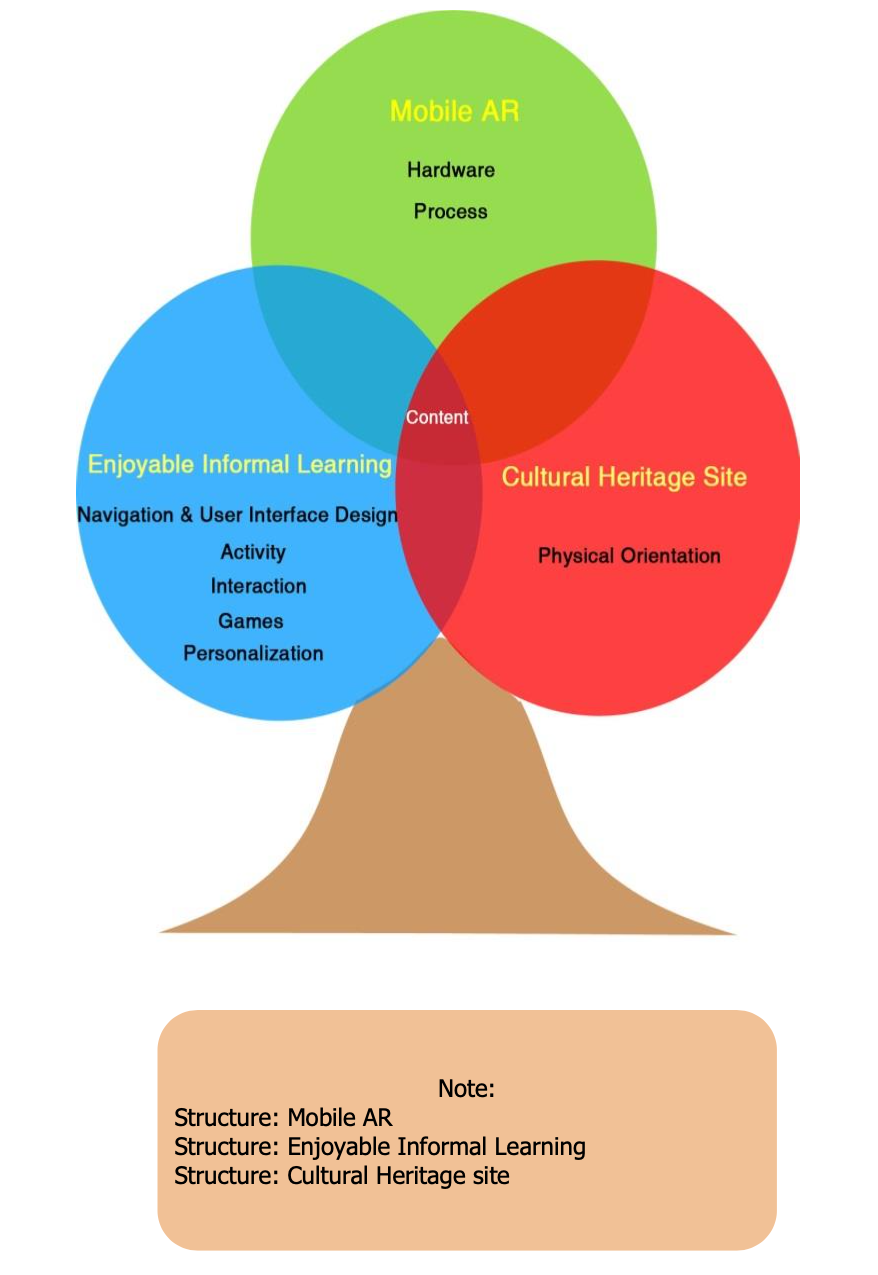
\includegraphics[width=8cm]{Figures/Background/models/ChandiniP.png}
    \caption{Conceptual Models - MARCHSTEIL}
    \label{fig:chandini}
\end{figure}

% AR + VR
Many efforts have been dedicated to include both VR and AR technologies. The approach presented in \cite{geiger_structured_2001} includes a design methodology for 3D environments that requires to be based on the metaphor of the actors whose actions correspond to a change in their attributes. It includes a 3D content library where the components of the environment are defined at a high level, is also extendable with third parties and independent of the operating system. The consequence of using a specific semantics such as actor roles does not allow the application of domain knowledge and forces the use of the framework provided by them.

Flotynski et al.~\cite{flotynski_conceptual_2015, flotynski_ontology-based_2017} also address semantic creation and modelling of 3D content in several studies. The SEMIC approach is presented as the combination of two elements: the SMC \cite{flotynski_semantic_2014, flotynski_semantic_2013, van_der_aalst_conceptual_2013}, on one hand, modelled as a collection of ontologies, which distinguishes concrete aspects such as geometry, space, structure, appearance, animation, behaviour and provides a representation of content at different levels of abstraction. The SCCM model \cite{mohler_semantic_2013}, on the other, translates the concepts of the SMC into their final representation through several steps, some of which are user-driven and others are performed automatically.

% XR & MR
The literature dealing with the modelling of mixed experiences is quite modest, yet of high relevance. They represent an important challenge for designers and developers, who need a tool able to define interaction techniques valid for multiple types of input devices. Gomes et al.~\cite{gomes_extended_2020} developed a toolkit to support the creation of applications and interaction techniques in VR, AR and MR. It also contains a set of literature-based resources including completely reviewed design methods, guidelines and frameworks, accessible via a web interface and useful to the user for the XR application development process. The design process consists of six phases and is executed iteratively, also covering a selection of several XR frameworks, a library of interaction techniques and a phase-by-phase analysis of potential pitfalls and issues that may be encountered during the course of the process.

% scripting language and formal language
Some of the works reviewed have also developed scripting languages and descriptive languages together with a conceptual model. An example of a language based on XML schema is VR-BML \cite{walczak_structured_2008-1}, it has two main types of commands, one related to the script structure and one operational. The scripts are leveraged for the dynamic creation of VR components arranged on the Beh-VR method \cite{hutchison_beh-vr_2006}.

Figueroa et al.~\cite{figueroa_conceptual_2006} provide formal specifications for the 3D interface components of MR experiences with respect to the device used, the modalities, the application type, the target group, the relationships between components and their behaviour. Furthermore, in parallel to the formal description of 3D Interaction Components, the authors propose the ICDL, a support tool, also based on XML. The work, though, does not delve into the aspects related to user tasks and skills.

Chevallier et al.~\cite{chevaillier_semantic_2012} implement another framework (\autoref{fig:chevaillier}) based on a standard notation, precisely the UML metamodel, with several additional extensions in order to apply it to the VR domain. The choice of using an already well-known modelling language is due to the clear mechanism and the possibility to provide the necessary abstraction for both content and system oriented semantic modelling. In \cite{costabile_formal_2005} the discussed advantage of formal descriptions compared to informal ones, that can bring unwanted unforeseen events, has resulted in the definition of a formalism called ICO to support multimodal interaction techniques. Encapsulating concepts from object-oriented programming (OOP), an object is an entity through which the behaviour of an ICO can be modelled, its appearance and interactions with users can be described.

\begin{figure}[h]
    \centering
    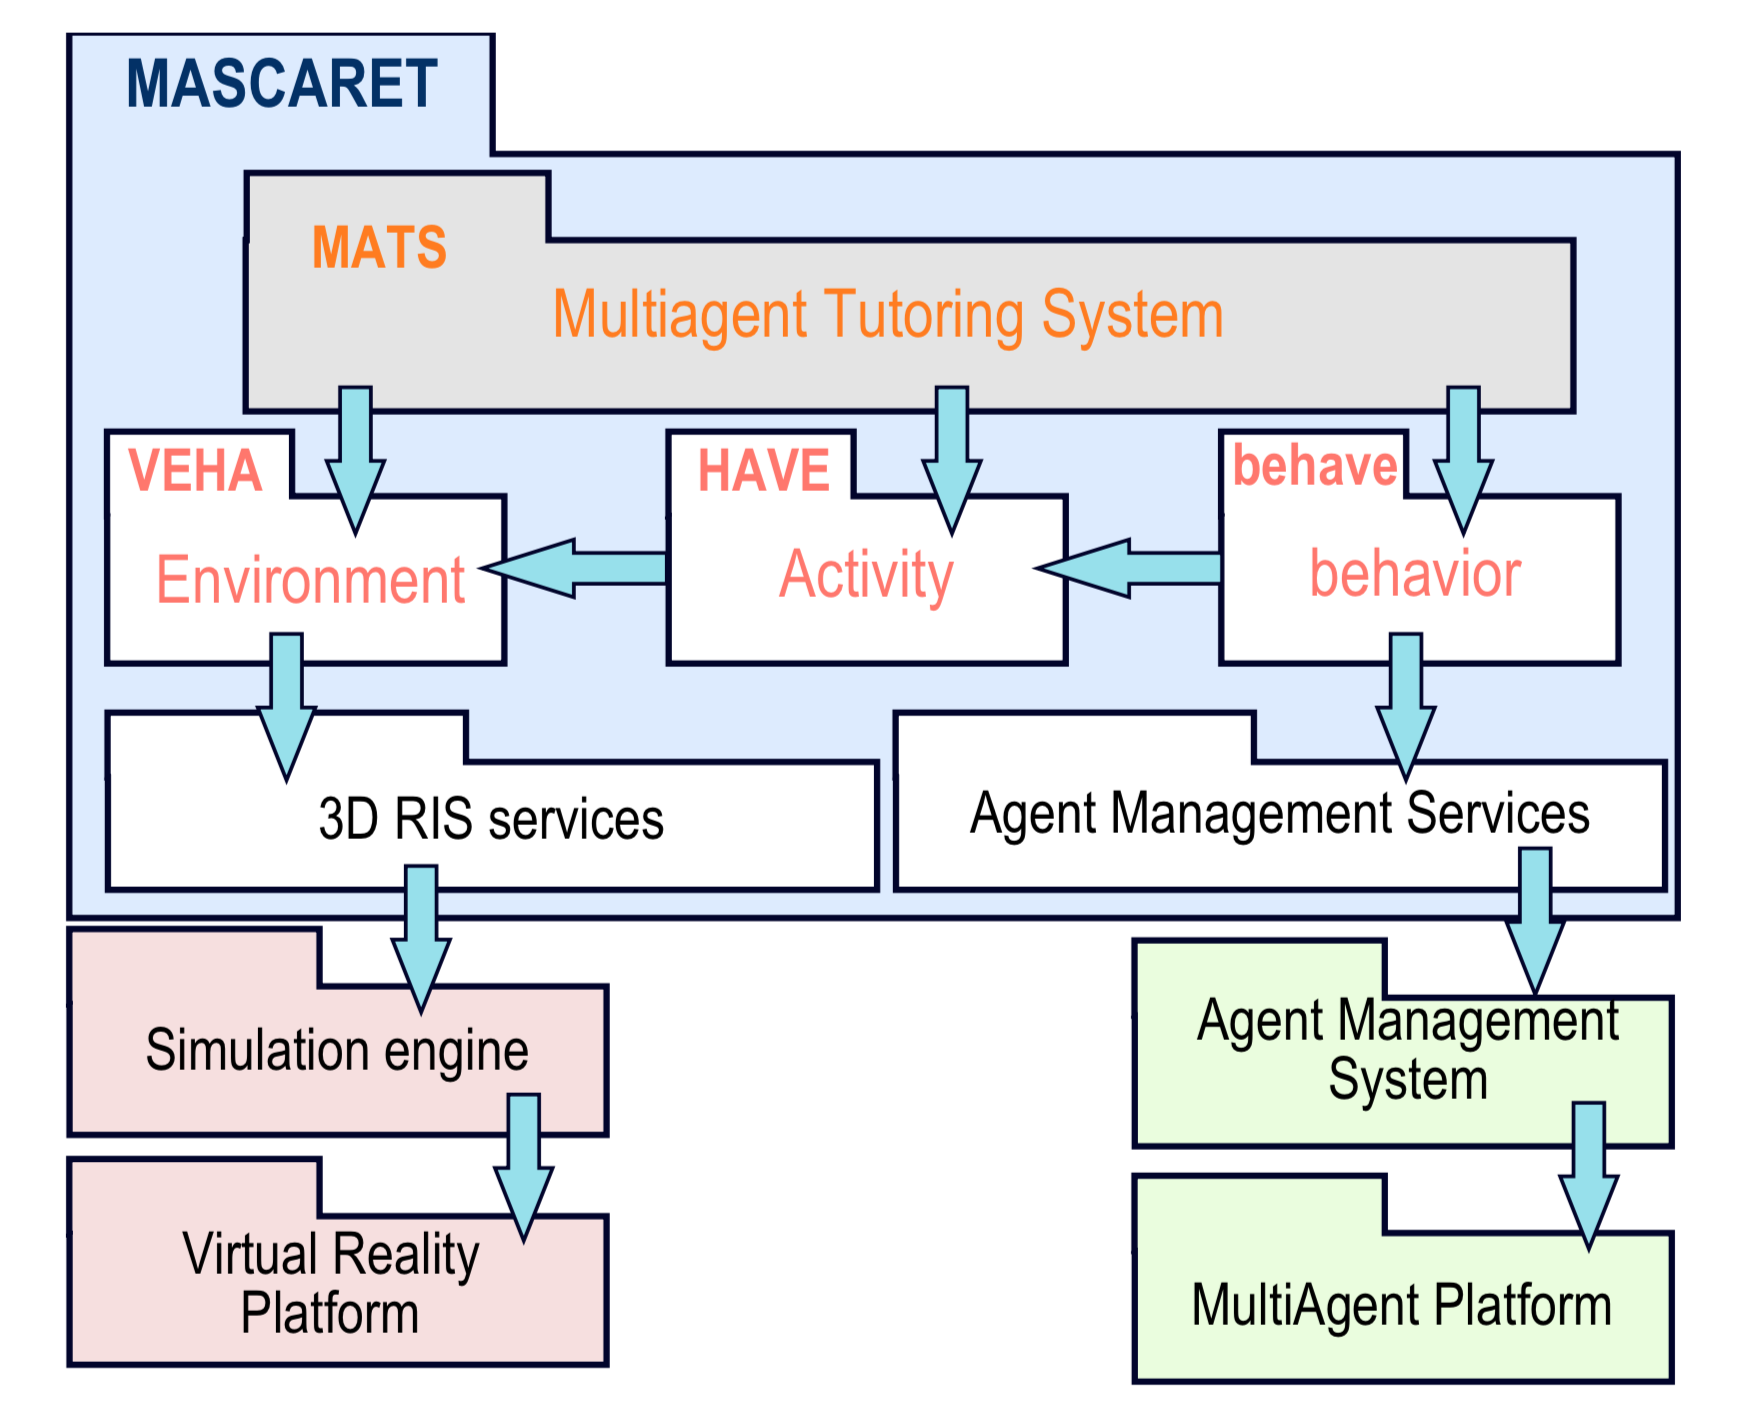
\includegraphics[width=12cm]{Figures/Background/models/chevallier.png}
    \caption{Conceptual Models - MASCARET}
    \label{fig:chevaillier}
\end{figure}

Multimodal interaction techniques are the subject of the event state-driven graphical notation (\autoref{fig:vanacken}) presented by Vanacken et al.~\cite{vanacken2006nimmit}. The primitives that constitute it are states and events, the task chain that must be executed, the data that these carry through states, the transition and conditional states, the hierarchical usage and the input/output parameters.  Even in this case, a framework based on the XML schema is attached to encapsulate the primitives and execute the interactions.

\begin{figure}[h]
    \centering
    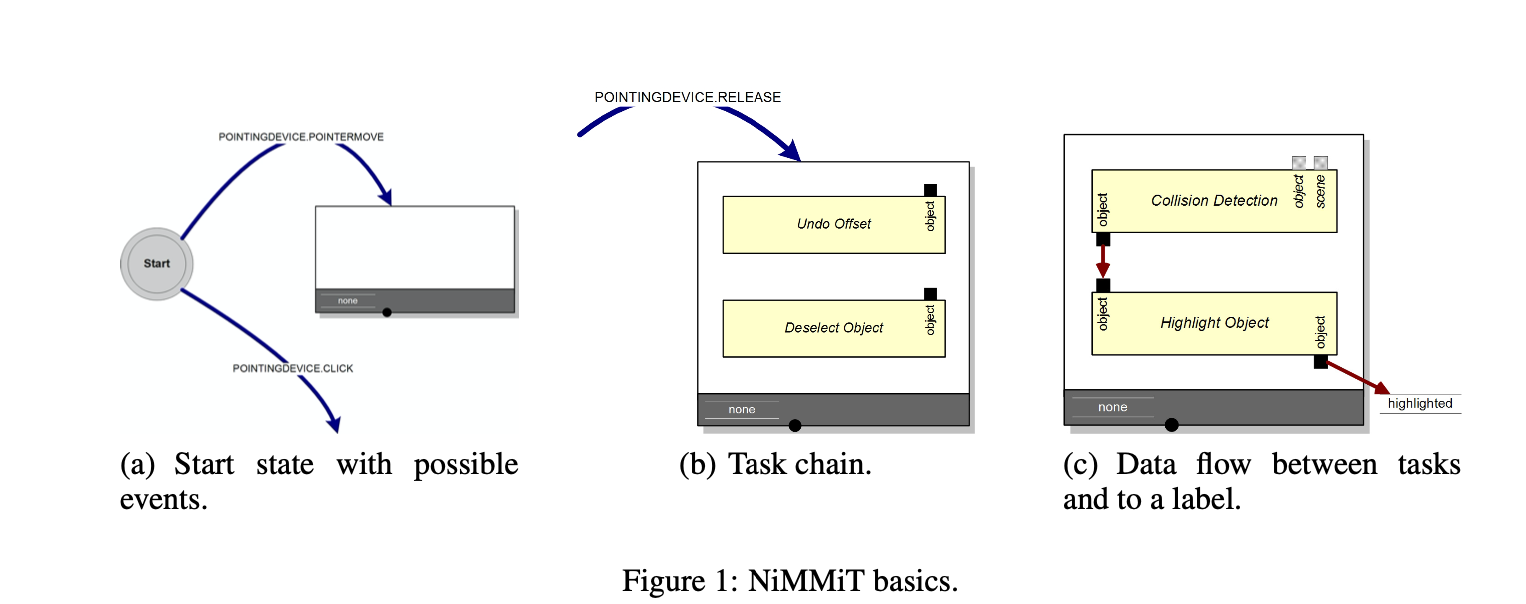
\includegraphics[width=\linewidth]{Figures/Background/models/vanacken1.png}
    \caption{Conceptual Models - NiMMiT}
    \label{fig:vanacken}
\end{figure}

Although it does not include any of the technologies relevant to this thesis, we believe it is crucial to mention the work carried out by Gianotti et al~\cite{dobbie_modeling_2020}. The conceptual model is applied to ISS, systems consisting of smart resources based on IoT devices, physical objects and software services that support human interactions. It comprises two sub-models (\autoref{fig:gianotti}), one used to describe the structural features and the other, instead, to define the behaviours and interactions between the actors that participate in the experience created for the ISS. 

\begin{figure}[h]
    \centering
    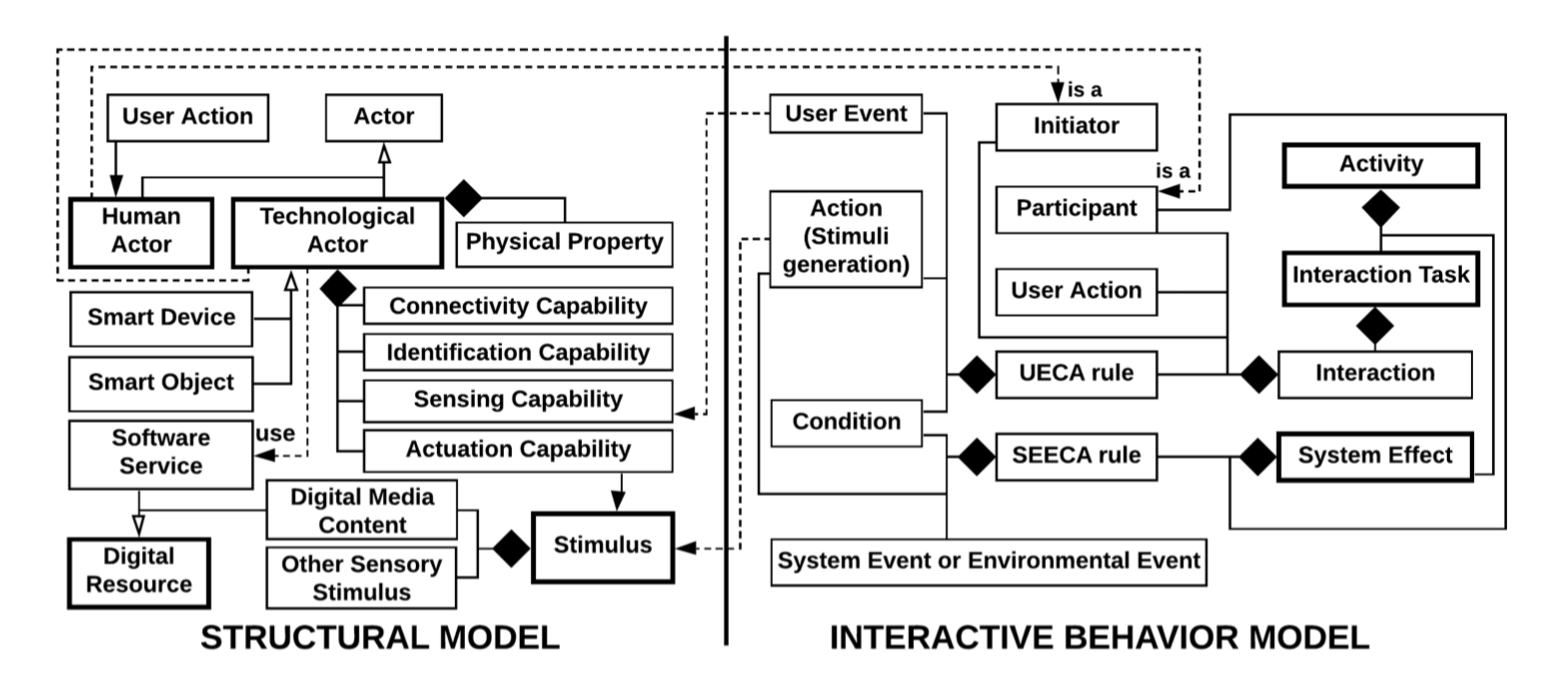
\includegraphics[width=\textwidth]{Figures/Background/models/gianotti.png}
    \caption{Conceptual Models - ISS Model}
    \label{fig:gianotti}
\end{figure}

\subsection{Comparative study}

After reviewing the numerous articles related to the study that is the subject of this thesis, it was decided to narrow down the overview of conceptual models by selecting three works found in the literature.

The resulting analysis was relevant to underline the features, to understand the strengths and weaknesses of each of them so as to guide the proposal of this thesis. The tables below summarizes their main characteristics. 

\begin{table}[h]
\begin{tabular}{|p{2.5cm}|p{3cm}|p{3cm}|p{3cm}|} 
\hline % The line on top of the table
\textbf{Approach} 
& \textbf{VR-WISE} 
& \textbf{MASCARET}
& \textbf{ISS MODEL} \\ 
\hline
Standard Language
& No
& Yes
& No\\ 
\hline
Informal Language
& Yes
& No
& Yes\\ 
\hline
\end{tabular} 
\caption{Comparative study: Approach}
\label{table:Approach}
\end{table}

The starting point for this analysis is the modelling language \textit{Approach} (\autoref{table:Approach}) pursued by the three concerned studies. The one that most closely follows a standard language is MASCARET \cite{chevaillier_semantic_2012}, whose authors argue for basing their model on an existing metamodel such as UML \cite{fowler_uml_2000} rather than building a new one. Since it is an extensible language, it is no longer aimed exclusively at software engineering, given its widespread use and semantic clarity. Within the stated strengths, the potential for experts to implement platform-independent models in their domain clashes with one of the main challenges raised in De Troyer et al.~\cite{de_troyer_conceptual_2007}, which prompted them to define a new language that is also accessible to non-professional backgrounds. 
The most popular general purpose conceptual modelling languages such as ER \cite{chen_context-aware_2019} and ORM \cite{halpin_conceptual_1995} can only model the static features in the application domain. Even though the UML also provides diagrams for drawing dynamic systems that describe the behaviour of objects as well as their appearance, the mechanisms are cumbersome, the amount of notions being too large to risk of causing ambiguity. However, this did not lead the authors of VR-WISE to exclude principles recalling the definition of object types and classes, typical of OOP, like Concepts, properties and instances of concepts. 
As to Gianotti et al.~\cite{dobbie_modeling_2020}, it bypasses the use of a standard language and addresses the lack of attention to human-related aspects in the existing models (within ISS) by proposing a solution centered on perceived interaction at different levels of abstraction. In this regard, therefore, the aim is to provide a set of tools that can be understood and enjoyed by the user, the main protagonist of the experience. 

\begin{table}
\begin{tabular}{|p{2.75cm}|p{3cm}|p{3cm}|p{3cm}|} 
\hline % The line on top of the table
\textbf{Environment}
& \textbf{VR-WISE} 
& \textbf{MASCARET}
& \textbf{ISS MODEL} \\ 
\hline
VR
& Yes
& Yes
& No\\ 
\hline
AR
& No
& No
& No\\ 
\hline
XR
& No
& No
& No\\ 
\hline
Other
& No
& No
& ISS\\ 
\hline
\end{tabular} 
\caption{Comparative study: Environment}
\label{table:Environment}
\end{table}

The second criterion, crucial in conceiving this thesis, highlights the \textit{Environments} for which the models are designed (\autoref{table:Environment}). The most widely used technology is certainly VR since the number of applications is greater compared to AR, and the samples examined for our comparative analysis also demonstrate this. 
In the last two decades a large number of authoring platforms and programming libraries have been deployed to support application developers in VR. 

Some examples of conceptual modeling specific to the AR domain exist in the literature but are limited because they are too tied to a single technology and therefore not so versatile. A separate mention must be made of the ISS Model, dedicated to Smart Spaces as a place for interactive user experiences. Although the environment is quite different from the other two models analysed -- in terms of the technologies used (IoT systems) -- the proposed conceptual model will clarify its fundamental presence in this comparative study. 
Finally, the lack of works covering the whole XR spectrum hints at some of the main reasons for this thesis project, i.e., the need to design cross-reality experiences with the same language.

\begin{table}
\begin{tabular}{|p{2.5cm}|p{3cm}|p{3cm}|p{3cm}|} 
\hline % The line on top of the table
\textbf{Conceptual Modeling} 
& \textbf{VR-WISE} 
& \textbf{MASCARET}
& \textbf{ISS MODEL} \\ 
\hline
Form
& Yes
& Yes
& Yes\\ 
\hline
Functions
& Yes
& Yes
& Yes\\ 
\hline
Behavior
& Yes
& Yes
& Yes\\ 
\hline
Interaction
& No
& Yes
& Yes\\ 
\hline
\end{tabular} 
\caption{Comparative study: Conceptual Modeling}
\label{table:Conceptual Modeling}
\end{table}

The following \autoref{table:Conceptual Modeling} serves as an introduction for the subsequent in-depth overviews of the models under consideration. The attributes that compose it, chosen as observation parameters, are inspired by the modules in which VR applications are decomposed according to Kim et al.~\cite{kim_software_1998}. Their approach, even if not too recent, identifies in the design of applications a static part, to which the form module belongs, and a dynamic one, which includes the functions, behaviour and interaction modules. Each module, whose meaning is considered in an extended way, is used to describe in more detail the substructures of each of the three models, albeit covered with different metaphors and nuances. The only work that does not explore interaction modelling in depth is VR-WISE, which is limited when faced with intricate interactions and therefore not exhaustive. 

\begin{table}
\begin{tabular}{|p{2.2cm}|p{3.1cm}|p{3.1cm}|p{3.1cm}|} 
\hline % The line on top of the table
\textbf{Form} 
& \textbf{VR-WISE} 
& \textbf{MASCARET}
& \textbf{ISS MODEL} \\ 
\hline
Model
& Static Structure
& VEHA
& Structural Model \\ 
\hline
Structural Entity
& Instances of Concepts
& "EntityClass"
& Building blocks \\ 
\hline
Object
& Simple objects and Complex objects
& General concepts and Physical object
& Human and Technological Actors \\ 
\hline
Property
& Visual and non visual
& Topological 
& Physical and digital \\ 
\hline
\end{tabular} 
\caption{Comparative study: Form}
\label{table:Form}
\end{table}

The \textit{Form} module refers to the external aspect of the objects that make up the virtual world, to the properties, the relations that characterize them and covers for each of the models analyzed, a distinct structure (\autoref{table:Form}). By means of the \textit{Structural Entity} attribute we want to identify the world elements at a high level of abstraction. In the case of VR-WISE and MASCARET they coincide with paradigms quite familiar in the engineering field. 
In the Domain Specification phase De Troyer et al.~\cite{de_troyer_conceptual_2007} distinguish concepts and properties, while in the World Specification, the world is populated by instances of such concepts i.e. simple and complex VR-Objects. Similarly in \cite{chevaillier_semantic_2012} the concept of Class, coming from the UML meta-model, is broadened to that of "EntityClass", more suitable to describe an environment where real and virtual objects are combined. 
In the Structural model of Gianotti et al.~\cite{dobbie_modeling_2020} the typical building blocks of the ISS are identified with the idea of actor which can be a human actor such as the end user, e.g. the tour guide, the visitor or a technological actor distinguishable in smart device and smart object. 

\begin{table}
\begin{tabular}{|p{2.2cm}|p{3.1cm}|p{3.1cm}|p{3.1cm}|} 
\hline % The line on top of the table
\textbf{Function} 
& \textbf{VR-WISE} 
& \textbf{MASCARET}
& \textbf{ISS MODEL} \\ 
\hline
Model
& Behavioral Modeling
& VEHA
& Interactive Behavioral Model \\ 
\hline
Actions
& Primitives and Composite behaviors
& Activity chart
& User Actions, Interaction Capabilities \\ 
\hline
\end{tabular} 
\caption{Comparative study: Function}
\label{table:Function}
\end{table}

The second module identifies among the primitives of each conceptual model, the one that describes what is used by virtual objects to perform a behavior, either spontaneous or reaction (\autoref{table:Function}). In the ISS Model, actors are distinguished by their interaction capabilities, which for the human actor translate into user actions involving other technological actors. These, indeed, are able to detect and share signals with other actors, generate stimuli perceived by users and be univocally recognized by the system. Whereas in VR-WISE actions are grouped according to the level of action, depending on the influence and changes they can cause on the object or on the whole environment, in the MASCARET model there is no clear distinction between actions and behaviors. The methods, with a notation recalling programming, are associated to their own "EntityClass" and are executed through the activity diagrams. 

\begin{table}
\begin{tabular}{|p{2.2cm}|p{3.1cm}|p{3.1cm}|p{3.1cm}|} 
\hline % The line on top of the table
\textbf{Behavior} 
& \textbf{VR-WISE} 
& \textbf{MASCARET}
& \textbf{ISS MODEL} \\ 
\hline
Model
& Modeling Behavior 
& VEHA, HAVE
& Structural Model, Interactive Behavioral Model \\ 
\hline
Perspective
& Action-oriented
& Event-driven
& Event-driven \\ 
\hline
Triggered by who
& Actor as a placeholder for an object
& Entities of the VEs
& HA, System Event, Environmental Event \\
\hline
Triggered by means
& Context-Event, Time-Event, User-Event, Object-Event
& Event (State-Transition-Event rule)
& User Event, System Event, Environmental Event \\
\hline
Reaction
& Behaviour function
& Reactive behaviours
& System Effect \\
\hline
\end{tabular} 
\caption{Comparative study: Behaviour}
\label{table:Behaviour}
\end{table}

Introducing the \textit{Behaviour} module we want to explain how the \textit{Functions} described above are performed by objects, hence their evolution in time expressed through states, transitions and constraints (\autoref{table:Behaviour}). To this end, for each of the conceptual models compared, the attributes of the table represent the author or the entity triggering the action and/or the event triggering the behaviour. Extending the approach of the UML behaviour diagrams, the VEHA sub-model determines the behaviour of a system in terms of its change of state during execution. However, by associating "EntityClasses" to state machines, when they perceive an event, a "reactive behaviour" could be triggered moving the entity into the next state \cite{chevaillier_semantic_2012}. The ISS Model describes the \textit{Behaviour} by introducing an additional abstraction level where there is a construct called UECA, based on the format of ECA rules typical of database systems and event-driven architectures. The effect generated on the system is the response to events caused by the Environment or the System itself. In opposition to models based on the state machine approach, VR-WISE adopts a model centred on the actions that actors can perform. Events that invoke behaviours are grouped in four event types divided into context, time, user and object. 

\begin{table}
\begin{tabular}{|p{2.2cm}|p{3.1cm}|p{3.1cm}|p{3.1cm}|} 
\hline % The line on top of the table
\textbf{Interaction} 
& \textbf{VR-WISE} 
& \textbf{MASCARET}
& \textbf{ISS MODEL} \\ 
\hline
Model
& - 
& HAVE
& Interactive Behavioral Model \\ 
\hline
Activity
& -
& Activity Model as flow of all possible execution of actions by an organizational entity.
& Interaction Task and System Effect \\ 
\hline
\end{tabular} 
\caption{Comparative study: Interaction}
\label{table:Interaction}
\end{table}

The modeling of \textit{Interaction} involves activities between objects with the user or with other objects (\autoref{table:Interaction}). Except for the VR-WISE model, where interaction modeling is missing and for which the authors refer to a partner project \cite{coninx_vr-demo_2006}, some combinations are addressed in HAVE, which borrows the concepts of collaboration and organization already existing in UML. HAVE leverages the concepts defined in VEHA to describe activities as collaborative procedures between autonomous agents and the user. An approach that becomes more agent-oriented is also presented in the ISS model. It can indeed be noted that the focus is on the actors as initiators and participants, involved in the sequence of operations. The activity executed is then defined as a flow chart including the two most important moments of the interaction, the Interaction Task and the System Effect. The result is a specification that is independent of the technology that will see it implemented, reusable and testable even by the non-expert. To conclude, it can be stated that, in the light of this comparative analysis, the characteristics reported by Gianotti et al. were considered the most suitable as a starting point for an internal study. Their work, actually, includes part of the prerequisites taken into consideration in order to lay the foundations of a conceptual model that has been designed thinking of a range of experiences covering one or more technologies.